\documentclass[12pt]{article}
\usepackage[spanish]{babel}
\usepackage[utf8]{inputenc}
\usepackage{geometry}
\geometry{a4paper, margin=2.5cm}
\usepackage{graphicx}
\title{Sistema de Recomendación de Optativas Universitarias}
\author{Proyecto para Modelos Matemáticos Aplicados}
\date{Junio 2025}

\begin{document}
\maketitle

\section*{Resumen}
Este proyecto consiste en el desarrollo de un sistema inteligente para la recomendación personalizada de asignaturas optativas a estudiantes universitarios. Utiliza técnicas avanzadas de Procesamiento de Lenguaje Natural (NLP), extracción de etiquetas (tags), generación de embeddings semánticos y modelos de lenguaje (LLM) para analizar tanto los intereses de los estudiantes como las descripciones de los cursos, facilitando así la toma de decisiones académicas.

\section{Objetivo}
El objetivo principal de este proyecto es proporcionar una herramienta inteligente y automatizada que facilite la toma de decisiones académicas para estudiantes universitarios al momento de elegir asignaturas optativas. El sistema busca:

\begin{itemize}
    \item \textbf{Personalización:} Ofrecer recomendaciones de cursos alineadas con los intereses, habilidades, trayectorias y expectativas individuales de cada estudiante, utilizando técnicas avanzadas de procesamiento de lenguaje natural y aprendizaje automático.
    \item \textbf{Optimización del proceso de orientación:} Reducir la incertidumbre y el tiempo que los estudiantes dedican a explorar la oferta de optativas, presentando sugerencias relevantes y justificadas.
    \item \textbf{Apoyo a la diversidad de perfiles:} Adaptarse a distintos perfiles estudiantiles, desde quienes tienen intereses muy definidos hasta quienes buscan explorar nuevas áreas, permitiendo una exploración guiada y flexible.
    \item \textbf{Facilitar la gestión docente:} Permitir a los docentes registrar y editar cursos de manera sencilla, asegurando que la información esté siempre actualizada y disponible para el sistema de recomendación.
    \item \textbf{Transparencia y explicabilidad:} Brindar a los usuarios información clara sobre por qué se recomienda cada curso, mostrando los intereses y similitudes detectadas.
    \item \textbf{Escalabilidad y replicabilidad:} Servir como base para sistemas similares en otras instituciones o contextos, gracias a su diseño modular y extensible.
\end{itemize}

En resumen, el sistema pretende ser un puente entre la oferta académica y las aspiraciones de los estudiantes, promoviendo una experiencia educativa más satisfactoria, informada y personalizada.

\section{Funcionamiento General}
El sistema sigue un flujo de trabajo estructurado y automatizado que integra diversas etapas de procesamiento de datos, análisis semántico y recomendación personalizada. A continuación se detalla cada fase del funcionamiento general:

\begin{enumerate}
    \item \textbf{Preprocesamiento de datos:}
    \begin{itemize}
        \item Limpieza y normalización de los textos de estudiantes y cursos, eliminando caracteres especiales, acentos y unificando el formato para facilitar el análisis posterior.
        \item Conversión de los intereses y descripciones en formatos estructurados y homogéneos.
    \end{itemize}
    \item \textbf{Extracción de tags:}
    \begin{itemize}
        \item Utilización de técnicas de NLP (spaCy) para extraer palabras clave relevantes de las descripciones de cursos y de los intereses de los estudiantes.
        \item Sugerencia automática de etiquetas mediante modelos de lenguaje (LLM) como OpenRouter/mistral-7b-instruct, enriqueciendo el conjunto de tags con términos semánticamente relevantes.
        \item Integración de una lista de etiquetas predefinidas para facilitar la selección manual por parte de los usuarios.
    \end{itemize}
    \item \textbf{Generación de embeddings:}
    \begin{itemize}
        \item Conversión de los tags y descripciones en vectores semánticos (embeddings) utilizando modelos como distiluse-base-multilingual-cased-v1.
        \item Almacenamiento de los embeddings generados para cursos y estudiantes, optimizando el cálculo de similitud y permitiendo actualizaciones eficientes.
    \end{itemize}
    \item \textbf{Cálculo de similitud:}
    \begin{itemize}
        \item Cálculo de la similitud coseno entre los embeddings de cada estudiante y los de todos los cursos disponibles.
        \item Generación de una matriz de afinidad que cuantifica el grado de correspondencia entre cada estudiante y cada curso.
    \end{itemize}
    \item \textbf{Recomendación:}
    \begin{itemize}
        \item Para cada estudiante, el sistema rankea los cursos según la similitud calculada, presentando un listado personalizado de las optativas más afines a sus intereses y perfil.
        \item Las recomendaciones se actualizan automáticamente ante cualquier cambio en los datos de estudiantes o cursos.
        \item Se proporciona información explicativa sobre el motivo de cada recomendación, mostrando los intereses y similitudes detectadas.
    \end{itemize}
    \item \textbf{Gestión y actualización:}
    \begin{itemize}
        \item Los docentes pueden registrar y editar cursos, y los estudiantes pueden actualizar sus intereses y descripciones en cualquier momento.
        \item El sistema recalcula automáticamente los tags, embeddings y recomendaciones ante cualquier modificación, garantizando resultados actualizados y relevantes.
    \end{itemize}
    \item \textbf{Interfaz interactiva:}
    \begin{itemize}
        \item Toda la interacción se realiza a través de una interfaz web amigable (Streamlit), que permite a los usuarios gestionar su información, consultar cursos y recibir recomendaciones de manera sencilla y visual.
    \end{itemize}
\end{enumerate}

Este flujo integral asegura que el sistema sea robusto, flexible y capaz de adaptarse dinámicamente a los cambios en la oferta académica y en los intereses de los estudiantes.

\section{Componentes Principales}
\begin{itemize}
    \item \textbf{data/}: Contiene los datos de cursos y estudiantes, así como los embeddings y tags generados.
    \begin{itemize}
        \item \textbf{courses.csv} y \textbf{students.csv}: Archivos principales con la información base de cursos y estudiantes.
        \item \texttt{courses\_with\_tags.csv} y \texttt{students\_with\_tags.csv}: Versiones enriquecidas con etiquetas (tags) extraídas automáticamente.
        \item \texttt{predefined\_tags.py}: Lista de etiquetas predefinidas para la selección de intereses.
        \item \texttt{courses\_tags\_embeddings.pkl} y \texttt{students\_tags\_embeddings.pkl}: Embeddings semánticos generados para cursos y estudiantes.
        \item \texttt{models/}: Modelos de embeddings descargados (por ejemplo, distiluse-base-multilingual-cased-v1).
    \end{itemize}
    \item \textbf{src/}: Código fuente principal para todo el procesamiento y lógica del sistema.
    \begin{itemize}
        \item \textbf{data\_preprocessing.py}: Limpieza y normalización de textos, carga de datos.
        \item \textbf{tag\_extraction.py}: Extracción automática de tags usando NLP (spaCy).
        \item \textbf{tag\_ia\_suggestion.py}: Sugerencia de tags usando modelos de lenguaje (LLM) vía OpenRouter.
        \item \textbf{embeddings.py}: Generación y gestión de embeddings semánticos para tags y descripciones.
        \item \textbf{similarity.py}: Cálculo de similitud coseno entre embeddings de estudiantes y cursos.
        \item \textbf{recommender.py}: Lógica principal de recomendación y ranking de cursos personalizados.
        \item \textbf{run\_workflow.py}: Script que ejecuta el flujo completo de procesamiento, extracción de tags, embeddings y recomendaciones.
        \item \textbf{utils.py}: Funciones auxiliares para carga y manipulación de datos.
        \item \textbf{api/elective\_recommendation.py}: API de alto nivel para registrar, editar y consultar estudiantes/cursos, y recalcular recomendaciones.
    \end{itemize}
    \item \textbf{app/}: Interfaz de usuario basada en Streamlit para interacción con estudiantes y docentes.
    \begin{itemize}
        \item \textbf{webapp.py}: Aplicación web principal, permite registrar, editar, consultar y recomendar cursos y estudiantes desde una interfaz amigable.
    \end{itemize}
    \item \textbf{README.md}: Documentación general y guía de uso del proyecto.
    \item \textbf{documentation/}: Documentación formal en formato \LaTeX{}.
\end{itemize}

\section{Tecnologías Utilizadas}
El sistema integra diversas tecnologías modernas de ciencia de datos, procesamiento de lenguaje natural y desarrollo web para lograr recomendaciones personalizadas y eficientes. A continuación se describen en detalle:

\begin{itemize}
    \item \textbf{Python}: Lenguaje principal de desarrollo, elegido por su ecosistema científico y de machine learning.
    \item \textbf{pandas}: Manipulación y análisis eficiente de datos tabulares (cursos, estudiantes, tags, embeddings).
    \item \textbf{sentence-transformers}: Biblioteca para generar embeddings semánticos de frases y palabras. Se emplea el modelo multilingüe `distiluse-base-multilingual-cased-v1` para representar los intereses y descripciones en un espacio vectorial.
    \item \textbf{spaCy}: Procesamiento de lenguaje natural en español, extracción de palabras clave (tags) mediante lematización y análisis gramatical.
    \item \textbf{Streamlit}: Framework para construir la interfaz web interactiva, permitiendo a estudiantes y docentes interactuar con el sistema de manera sencilla y visual.
    \item \textbf{OpenRouter/mistral-7b-instruct}: Modelo de lenguaje grande (LLM) accesible vía API, utilizado para sugerir automáticamente etiquetas relevantes a partir de descripciones de cursos, enriqueciendo el sistema de tags.
    \item \textbf{dotenv}: Gestión de variables de entorno, como claves de API para servicios externos.
    \item \textbf{HuggingFace Hub}: Descarga y gestión de modelos preentrenados de embeddings.
\end{itemize}

Estas tecnologías permiten combinar procesamiento lingüístico avanzado, aprendizaje automático y una experiencia de usuario moderna, logrando un sistema robusto y flexible para la recomendación de optativas universitarias.

\section{Interfaz de Usuario}
La interfaz de usuario está implementada con Streamlit y permite la interacción tanto para estudiantes como para docentes de manera sencilla e intuitiva. A continuación se detallan sus funcionalidades principales:

\begin{itemize}
    \item \textbf{Selección de rol}: Al iniciar la aplicación, el usuario puede elegir entre los roles de Estudiante o Docente desde la barra lateral.
    \item \textbf{Opciones para Estudiantes}:
    \begin{itemize}
        \item \textbf{Registrar}: Permite a un nuevo estudiante registrarse, ingresando su nombre, seleccionando intereses desde una lista de etiquetas predefinidas y describiendo sus expectativas. Los datos se almacenan y procesan automáticamente.
        \item \textbf{Editar información}: Un estudiante puede buscarse por su ID, cargar su información actual y modificar nombre, intereses o descripción. Los cambios se guardan y actualizan los datos procesados.
        \item \textbf{Consultar información}: Permite consultar los datos de cualquier estudiante ingresando su ID.
        \item \textbf{Ver cursos disponibles}: Muestra la lista de cursos registrados, con nombre, ID y descripción.
        \item \textbf{Recomendar cursos}: El estudiante ingresa su ID y el sistema muestra un ranking personalizado de cursos recomendados, calculado en tiempo real según sus intereses y los embeddings generados.
    \end{itemize}
    \item \textbf{Opciones para Docentes}:
    \begin{itemize}
        \item \textbf{Registrar curso}: Permite registrar un nuevo curso, ingresando nombre y descripción.
        \item \textbf{Editar curso}: Permite buscar un curso por ID, cargar su información y editar nombre o descripción.
        \item \textbf{Ver cursos disponibles}: Visualiza todos los cursos registrados, con detalles ampliados para docentes.
    \end{itemize}
    \item \textbf{Interacción y validación}: La interfaz valida los campos obligatorios (por ejemplo, nombre no vacío) y muestra mensajes de éxito o error según la acción realizada.
    \item \textbf{Actualización dinámica}: Los formularios y listados se actualizan dinámicamente según las acciones del usuario, garantizando una experiencia fluida.
\end{itemize}

Toda la lógica de la interfaz se encuentra en el archivo \texttt{app/webapp.py}, que conecta la capa visual con la API de recomendación y los módulos de procesamiento de datos. Esto permite que tanto estudiantes como docentes gestionen y consulten información, y accedan a recomendaciones personalizadas de manera centralizada y amigable.

\section{Casos de Uso}
A continuación se describen los principales casos de uso del sistema, detallando el flujo y las acciones involucradas en cada uno:

\begin{itemize}
    \item \textbf{Registro de un nuevo estudiante:}
    \begin{itemize}
        \item El usuario selecciona el rol de Estudiante y elige la opción "Registrar".
        \item Completa un formulario con su nombre, selecciona intereses desde una lista de etiquetas predefinidas y puede agregar una descripción personalizada de sus expectativas.
        \item Al enviar el formulario, el sistema valida los datos y almacena la información en la base de datos (archivo CSV), generando automáticamente los tags y embeddings asociados.
        \item El estudiante queda registrado y listo para recibir recomendaciones personalizadas.
    \end{itemize}
    \item \textbf{Edición de información de estudiante:}
    \begin{itemize}
        \item El estudiante ingresa su ID y carga su información actual.
        \item Puede modificar su nombre, intereses o descripción.
        \item Al guardar los cambios, el sistema actualiza los datos y recalcula los embeddings y recomendaciones asociadas.
    \end{itemize}
    \item \textbf{Consulta de información de estudiante:}
    \begin{itemize}
        \item Permite a cualquier usuario consultar los datos de un estudiante ingresando su ID.
        \item Se muestra la información registrada, incluyendo intereses y descripción.
    \end{itemize}
    \item \textbf{Visualización de cursos disponibles:}
    \begin{itemize}
        \item Tanto estudiantes como docentes pueden ver la lista completa de cursos registrados.
        \item Se muestran detalles como nombre, ID y descripción de cada curso.
    \end{itemize}
    \item \textbf{Recomendación personalizada de cursos:}
    \begin{itemize}
        \item El estudiante ingresa su ID y solicita recomendaciones.
        \item El sistema calcula la similitud entre los intereses del estudiante y los cursos disponibles usando embeddings y similitud coseno.
        \item Se muestra un ranking de los cursos más recomendados, junto con el puntaje de afinidad y detalles de cada curso.
    \end{itemize}
    \item \textbf{Registro y edición de cursos (Docente):}
    \begin{itemize}
        \item El docente puede registrar un nuevo curso ingresando nombre y descripción, o editar un curso existente buscando por ID.
        \item Los cambios se reflejan en la base de datos y se actualizan los tags y embeddings del curso automáticamente.
        \item Los cursos editados o nuevos quedan disponibles para ser recomendados a los estudiantes.
    \end{itemize}
\end{itemize}

Estos casos de uso cubren los principales flujos de interacción previstos en la plataforma, asegurando una experiencia completa tanto para estudiantes como para docentes.

\section{Requisitos}
\begin{itemize}
    \item Python 3.8 o superior
    \item Dependencias listadas en requirements.txt:
    \begin{itemize}
        \item pandas
        \item sentence-transformers
        \item spacy
        \item flask
        \item streamlit
        \item dotenv
        \item requests
        \item huggingface-hub
    \end{itemize}
    \item Acceso a internet para usar la API de OpenRouter (opcional, solo para sugerencia automática de tags)
\end{itemize}



\section{Validación Experimental}

La validación experimental del sistema se estructura en torno a los siguientes aspectos clave: extracción de etiquetas (tags) y recomendaciones personalizadas.

\subsection{Extracción de Tags}

\textbf{Ejemplo de Cursos:}

\begin{itemize}
    \item \textbf{Curso:} Inteligencia Artificial\\
    \textbf{Descripción:} Introducción a los conceptos y técnicas de IA, aprendizaje automático, redes neuronales y aplicaciones.\\
    \textbf{Tags extraídos (NLP):} aprendizaje, red, inteligencia, aplicación, concepto\\
    \textbf{Tags IA (LLM):} inteligencia artificial, machine learning, redes neuronales, automatización, aprendizaje automático

    \item \textbf{Curso:} Criptografía\\
    \textbf{Descripción:} Este curso explora los principios matemáticos detrás de la criptografía moderna, incluyendo algoritmos de cifrado, funciones hash y protocolos de seguridad.\\
    \textbf{Tags extraídos (NLP):} criptografia, algoritmo cifrado, algoritmo, cifrado, función, hash, protocolo, seguridad\\
    \textbf{Tags IA (LLM):} criptografía, seguridad, cifrado, funciones hash, protocolos
\end{itemize}

\subsection{Ejemplo de Estudiantes}

\begin{itemize}
    \item \textbf{Estudiante:} Valentina\\
    \textbf{Descripción:} Me apasiona el big data y la ciencia de datos. Quiero mejorar mis habilidades en estadística y visualización.\\
    \textbf{Intereses:} big data, analisis de datos, estadistica, visualizacion, ciencia de datos\\
    \textbf{Tags extraídos:} analisis de dato, big, big datar, ciencia, ciencia de dato, data, dato, estadistica, estadisticar, visualizacion

    \item \textbf{Estudiante:} Martí\\
    \textbf{Descripción:} Me interesaría saber cómo funciona el internet y las redes de computadoras.\\
    \textbf{Intereses:} redes\\
    \textbf{Tags extraídos:} computadora, internet, red
\end{itemize}

\subsection{Recomendación}

%\textbf{Matriz de Similitud Coseno:}
\begin{center}
    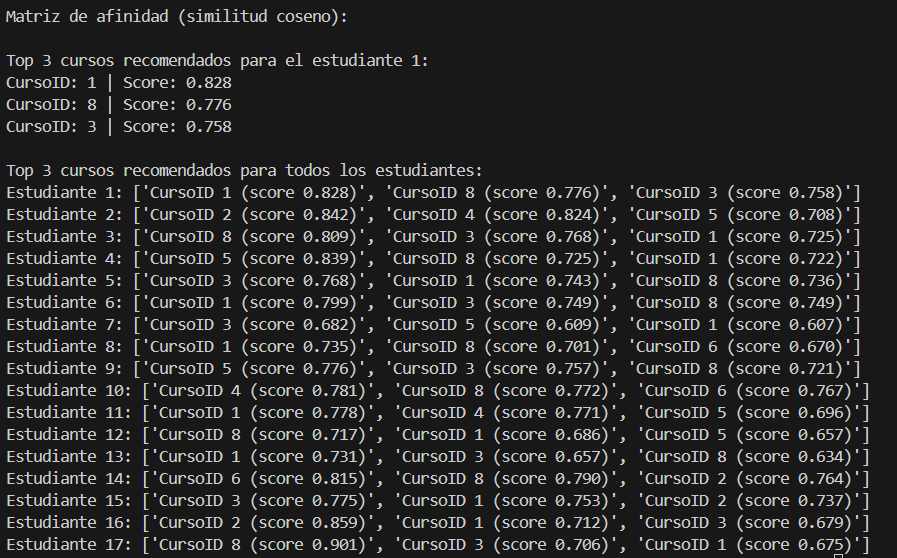
\includegraphics[width=0.9\textwidth]{recomendaciones.png}
\end{center}

\textbf{Top Recomendaciones para Estudiantes:}

\begin{itemize}
    \item \textbf{Estudiante:} Valentina\\
    \textbf{Cursos recomendados:}
    \begin{enumerate}
        \item Matemática Discreta (ID: 3) -- Score: 0.809\\
        Lógica, conjuntos, grafos y combinatoria para ciencias de la computación.
        \item Base de Datos (ID: 5) -- Score: 0.782\\
        Modelado, diseño y administración de bases de datos relacionales y no relacionales.
        \item Optimización (ID: 8) -- Score: 0.763\\
        Este curso se enfoca en técnicas para encontrar el mejor resultado en problemas matemáticos, como programación lineal y no lineal, algoritmos genéticos y optimización convexa.
    \end{enumerate}

    \item \textbf{Estudiante:} Martí\\
    \textbf{Cursos recomendados:}
    \begin{enumerate}
        \item Redes de Computadoras (ID: 2) -- Score: 0.838\\
        Estudio de protocolos, arquitecturas y seguridad en redes de computadoras.
        \item Inteligencia Artificial (ID: 1) -- Score: 0.712\\
        Introducción a los conceptos y técnicas de IA, aprendizaje automático, redes neuronales y aplicaciones.
        \item Matemática Discreta (ID: 3) -- Score: 0.698\\
        Lógica, conjuntos, grafos y combinatoria para ciencias de la computación.
    \end{enumerate}
\end{itemize}

\section{Créditos}
Desarrollado para la asignatura de Modelos Matemáticos Aplicados.

\end{document}
